\section{问题背景}

古代丝绸之路不仅是商贸通道,也是文化与技术交流的重要桥梁,其中,玻璃制品是早期东西方物质文化交流的重要物证。早期玻璃制品由西亚和埃及地区传入,其技术与风格影响了中国本土的玻璃制造业。中国古代工匠在吸收外来技术的基础上,利用本土原料进行生产,制造出外观相似但化学成分体系相异的玻璃器物。这种成分上的差异为鉴别古代玻璃制品的产地与技术来源提供了客观依据。

玻璃的主要成分为二氧化硅 ($SiO_2$)。为降低其熔点,制造过程中需加入助熔剂。古代中西方采用的助熔剂体系不同,形成了成分各异的玻璃类别。例如,以草木灰为助熔剂的钾玻璃 ($K_2O$ 含量较高) 和以铅矿石为助熔剂的铅钡玻璃 ($PbO$、$BaO$ 含量较高),后者被普遍认为是古代中国独立发展的玻璃品种。然而,玻璃制品在长期埋藏过程中,其表面易与环境发生元素交换,导致化学成分发生改变,这一风化过程给准确的成分分析与类型鉴别带来了挑战。因此,需要建立一套系统的数据分析方法,以消除或减弱风化作用的干扰,准确识别玻璃文物的化学成分规律,并对其进行科学分类与鉴别。


% \begin{figure}[htbp]
%     \centering
%     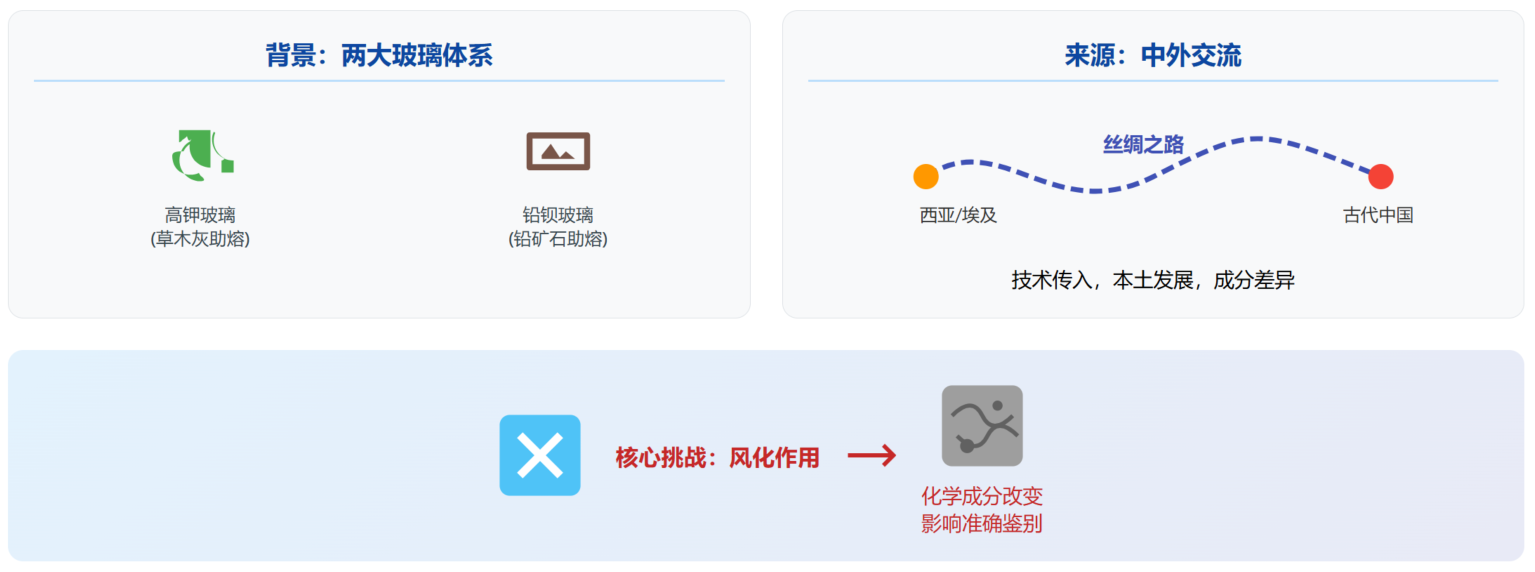
\includegraphics[width=\textwidth]{figs/1前置/问题背景.png}
%     \caption{问题背景} 
%     \label{fig:your_image_label} 
% \end{figure}


\section{问题重述}

问题一:分析玻璃文物表面风化状态与其玻璃类型、纹饰和颜色等物理属性的统计关系。在此基础上,结合玻璃类型,研究表面风化对化学成分含量的影响规律,并建立数学模型,根据风化样品的化学成分数据,预测其风化前的成分含量。

问题二:根据已分类的高钾玻璃与铅钡玻璃的化学成分数据,建立有效的分类判据。进而,在每个大类中,选择合适的化学成分作为指标,对该类别进行亚类划分,并给出具体的划分方案。最后,对分类与划分结果的合理性及稳定性进行分析。

问题三:利用已建立的分类模型,对一批未知类别的玻璃文物样品的化学成分数据进行分析,鉴别其所属的玻璃类型。同时,需要对鉴别结果的敏感性进行评估,以考察分类结果的稳健程度。

问题四:针对高钾玻璃与铅钡玻璃两个类别,分别探究其内部各化学成分之间的关联关系。通过比较两个类别在化学成分关联模式上的异同,表现不同玻璃体系在原料构成与制造工艺上可能存在的差异。

\section{问题分析}

对于问题一,该问题包含两个递进的部分。第一部分要求分析风化状态与玻璃类型、纹饰、颜色等多个定性变量之间的关系,可采用列联表分析与卡方检验等统计方法,检验这些变量之间是否存在显著的相依性。第二部分旨在建立风化前后化学成分的映射关系。此过程可视为一个回归或预测问题,可以通过分析同一文物上风化点与未风化点的成分差异,建立多元回归模型,从而实现对风化前成分的定量估计。

对于问题二,其核心是分类与聚类任务。首先,区分高钾与铅钡玻璃是一个监督学习分类问题。由于类别标签已知,可利用逻辑回归、支持向量机或决策树等分类算法,建立基于化学成分的分类器。其次,在已确定的类别内部进行亚类划分,是一个无监督学习的聚类问题。因缺乏亚类的先验标签,可采用K-均值聚类或层次聚类等算法,依据关键化学成分的分布特征进行探索性划分。对结果的合理性分析可通过交叉验证评估分类器性能,通过轮廓系数等指标评价聚类效果;敏感性分析则可通过扰动数据来检验模型输出的稳定性。

对于问题三,该问题是问题二所建分类模型的直接应用。需要将表单三中未分类样本的化学成分数据输入已训练好的分类器,以获得其预测类别。其敏感性分析旨在评估分类决策的可靠性,可以通过计算样本点到分类边界的距离或在样本成分数据上施加微小扰动,观察分类结果是否发生改变,来衡量分类的稳健性。

对于问题四,该问题要求探究不同类别玻璃内部化学成分的相互关系。此分析可通过计算各类别样本的协方差矩阵或相关系数矩阵来实现。皮尔逊相关系数是衡量两个连续变量间线性关系强度的常用指标。通过为高钾和铅钡玻璃分别构建相关系数矩阵,并利用热力图等可视化手段,可以直观地展示不同类别玻璃内部各元素间的协同或拮抗关系,比较其模式差异,为探究其工艺与原料来源提供数据支持。
